\subsection{Protocollo di comunicazione}
In generale, il protocollo di comunicazione prevede che il client invii messaggi di comando in cui venga specificato il tipo di comando da eseguire, il server, quindi esegue il comando e invia un messaggio di risposta.\\
Ogni comando prevede un trasferimento file, quindi, a seconda del tipo di comando, o nel messaggio di comando o in quello di risposta viene allegato il file, con le informazioni necessarie alla sua corretta ricezione.\\
Ogni messaggio di comando e di risposta è composto da campi di un numero fissato di byte contenenti le informazioni necessarie all'interpretazione del messaggio.
Essendo un'applicazione distribuita, i campi vengono distinti utilizzando variabili la cui ampiezza (numero di bit) è indipendente dall'architettura della macchina, a tal proposito ogni campo informativo è composto dalle variabili definite in \emph{stdint.h}.\\ 
I primi 8 bit di un messaggio di comando indicano sempre il tipo di comando da eseguire e, a seconda del comando, possono avere o meno ulteriori informazioni.

\begin{lstlisting}[title=Costanti comandi]
// command codes
#define LIST 		0
#define GET 		1
#define PUT 		2

// response codes
#define GET_OK      0
#define GET_NOENT   1
#define PUT_SUCCESS 2
#define PUT_FAILURE 3
\end{lstlisting}

%\begin{figure}
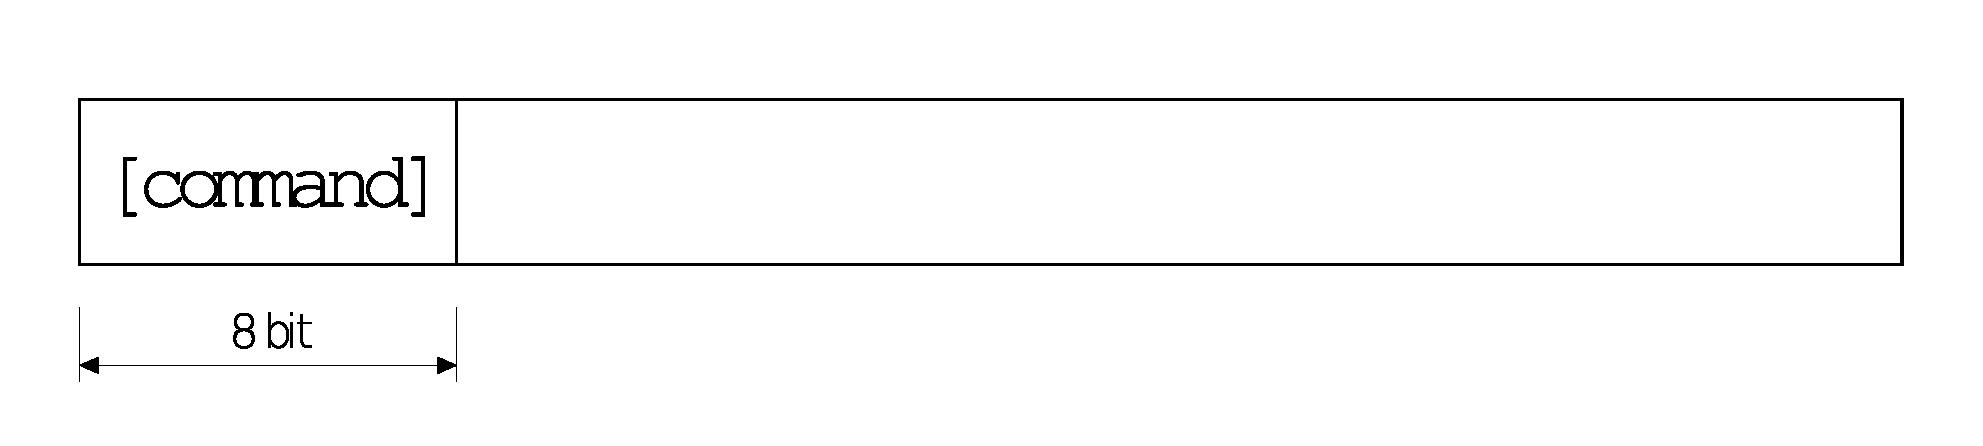
\includegraphics[scale=0.35]{images/gen_message}
%\end{figure}

Una volta impostati i vari campi in un buffer, se non va inviato un file, i dati vengono passati direttamente al livello di trasporto virtuale.\\
Se altrimenti, va inviato un file, viene chiamata la funzione \emph{send\_file}, i campi informativi vengono considerati un header per il file ed il tutto viene frammentato (per non allocare troppa RAM) e passato al livello sottostante.\\
Lato opposto il ricevente analizza uno alla volta i campi informativi, poi legge il file tramite la funzione \emph{recv\_file}.


\begin{lstlisting}[title=cmd\_commons.c]
void send_file(int fd, void *header, size_t file_size, 
				size_t header_size)								
{                                                                                                       
	int8_t buffer[MAX_BUFSIZE];                                                                         
	size_t buf_size, total_size;                                                                        
	unsigned int i, n;                                                                                  
																										
	total_size = header_size + file_size;                                                               
	n = total_size / MAX_BUFSIZE;                                                                       
																										
	memcpy(buffer, header, header_size);                                                                
																										
	for (i = 0; i <= n; i++) {                                                                          
																										
		// calculate last bytes to send                                         
		if (i == n) {           
			buf_size = total_size % MAX_BUFSIZE;                                                        
			if (!buf_size)                                                                              
				// total size is a multiple of MAX_BUFSIZE:
				// send only n-1 chunks        
				break;          
		} else                                                                                          
			buf_size = MAX_BUFSIZE;                                                                     
																										
		if (readn(fd, buffer + header_size, buf_size - header_size)
			== -1)                              
			handle_error("readn() - reading file to send");

		header_size = 0;  // consider header only at the first pass

		rdt_send(buffer, buf_size);
	}
}

void recv_file(int fd, size_t size)
{
	unsigned int i, n = size / MAX_BUFSIZE;
	size_t buf_size;
	int8_t buffer[MAX_BUFSIZE];
                                                                                              
	for (i = 0; i <= n; i++) {
                                                                                              
		// calculate last bytes to store 
		if (i == n) {           
			buf_size = size % MAX_BUFSIZE;
			if (!buf_size)
				// size is a multiple of MAX_BUFSIZE:
				// receive only n-1 chunks
				break;          
		} else
			buf_size = MAX_BUFSIZE;
                                                                                              
		rdt_recv(buffer, buf_size);
                                                                                              
		if (writen(fd, buffer, buf_size) == -1)
			handle_error("writen() - writing received file");
	}
}
\end{lstlisting}
